\chapter{Results}
\section{Water Year 2019} 
\subsection{Thermocouple Array}
The instrument was installed and fully operational on November 16, 2018 and collected continuous temperature measurements for the whole season. Some challenges from this winter include: (i) sagging of the support cables, (ii) snow bridging between vertical steel supports causing a deeper snow profile, (iii) snow depths exceeded the height of our sensor, (iv) some thermocouples are functioning intermittently after the major snowfall in February, and (iv) channelized/irregular melt patterns around the structure of the sensor in the spring. Despite the above challenges, this dataset suggests that it is possible to use this instrument as a tool for measuring the temperature profile of a snowpack. 

Throughout the season, as snow accumulates, the settling snowpack applies an increasing downward force on the sensor. As a result, some of the support cables sag a few centimeters. The cables also act as a support for the snowpack, so as the snow settles, there is often an elevated snow surface at the temperature array. This promotes the growth of a snow bridge between the two vertical supports. This bridging effect is observable in this data when comparing the snow depth to the temperature profile.   

Thermocouples buried in the soil and at the ground surface consistently read about 0\textdegree C (Figure \ref{fig:Soil_20cm_Accumulation}). Moving up through the snowpack, there is a consistent temperature gradient from the 0\textdegree C ground measurement to air temperature (Figure \ref{fig:25cm_55cm_Accumulation}). The array of thermocouples above the snowpack measure the same temperature and have much larger diurnal fluctuation than buried sensors (Figure \ref{fig:Dec_Jan_ImageSC}). The snowpack has a large damping effect on temperature fluctuations which makes it possible to estimate snow depth using the temperature profile. However, the snow bridging is clearly seen in this temperature damping and leads to overestimation of snow depth when using the temperature profile as a metric. 

\begin{figure}[H]
    \centering
    \includegraphics[width=0.9\linewidth]{figures/Soil_20cm_Accumulation.jpg}
    \caption{Temperature measurement for the thermocouple buried 10cm below ground up to the thermocouple 20cm above ground. At this point, they are all buried in snow.}
    \label{fig:Soil_20cm_Accumulation}
 \end{figure}

\begin{figure}[H]
    \centering
    \includegraphics[width=0.9\linewidth]{figures/25cm_55cm_Accumulation.jpg}
    \caption{Temperature measurements for the thermocouples between 25cm and 55cm above ground. Note the damping of temperature as the upper thermocouples become buried in snow.}
    \label{fig:25cm_55cm_Accumulation}
 \end{figure}
 
\begin{figure}[H]
    \centering
    \includegraphics[width=0.9\linewidth]{figures/Dec_Jan_ImageSC.jpg}
    \caption{Continuous plot of the temperature measurements between Nov 30th - Jan 18. The horizontal white line is the snow depth recorded by an acoustic sensor at the SNOTEL site. }
    \label{fig:Dec_Jan_ImageSC}
 \end{figure}

The precision and accuracy of this instrument is tested during isothermal conditions in the snowpack. During water year 2019, the snowpack went isothermal around March 31 (Figure \ref{fig:0_135cm_Isothermal}) and peak snowmelt started on April 16. This followed a couple warm storm events that deposited a few inches of snow in early April (Figure \ref{fig:SWE_SNTLTemp}). On average, the instrument over-estimates temperature by no more than 0.05\textdegree C (Figure \ref{fig:IsothermBoxplot}). As seen in Figure \ref{fig:IsothermBoxplot}, not every thermocouple behaves the same. One possible explanation for this is the aged Campbell Scientific AM32 Multiplexors that are used in the 2019 water year. These were later replaced because they failed during the 2019 summer.  
 
\begin{figure}[H]
    \centering
    \includegraphics[width=0.7\linewidth]{figures/SWE_SNTLTemp.jpg}
    \caption{Time series of SWE at Banner summit plotted with the observed air temperature at the SNOTEL site.}
    \label{fig:SWE_SNTLTemp}
\end{figure}

In the beginning of April, each buried thermocouple had very little daily temperature fluctuations (Figure \ref{fig:DailyTempRange}). Directly after peak snowmelt started, the daily range for each thermocouple increased greatly and in some cases is larger than 1\textdegree C. This increase in temperature fluctuation is likely caused by preferential flow of snowmelt due to the instrument. During the melt season, a channel formed between the two vertical supports creating a depression in the snow surface where the thermocouples are placed. Because the instrument has different thermal properties (e.g. albedo and thermal conductivity), it affects melt rates and characteristics of the snow it is in contact with. It is suspected that the instrument facilitates an increased downward flow of water which creates air pockets around the sensor that affect its ability to accurately measure snow temperature in the spring. 

\begin{figure}[H]
    \raggedleft
    \includegraphics[width=1\linewidth]{figures/Isotherm_boxplot.jpg}
    \caption{Average daily temperature for each thermocouple between -10cm to 60cm.}
    \label{fig:IsothermBoxplot}
 \end{figure}
 
 \begin{figure}[H]
    \centering
    \includegraphics[width=0.8\linewidth]{figures/DailyTempRange_Isotherm.jpg}
    \caption{The daily temperature range for each thermocouple between -10cm to 135cm.}
    \label{fig:DailyTempRange}
 \end{figure}
 
\subsection{Temperature Gradient Analysis}
Avalanche forecasters are primarily interested in the timing and duration of critical temperature gradients in the snowpack. Figure \ref{fig;WY2019_L20_Grad} shows temperature gradients in the lowest 20cm throughout the whole period of record. These results suggest that higher than critical temperature gradients persist throughout December, but there is no concern for temperature gradient metamorphism for the remainder of the season. Figures \ref{fig:Dec_U25_RDH} - \ref{fig:Dec_L20_RDH} display the relative frequency of temperature gradients during December in the upper and lower portions of the snowpack, respectively. Cold air temperatures during December forced above-critical temperature gradients on the shallow snowpack for nearly 50\% of the month. 

Figures  \ref{fig:Feb_U25_RDH} - \ref{fig:Feb_L20_RDH} show the mid-season analysis during February. By this point in the season, the lowest 20cm of the snowpack is well insulated; thus, there is little to no temperature gradient. Although the upper portion of the snowpack experiences substantial temperature gradients, they are not persistent because of the diurnal solar cycle. Because of this, temperature gradients were above critical in the upper 25cm for 14\% of February. 

Figures \ref{fig:Mar_U25_RDH} - \ref{fig:Mar_L20_RDH} show the late-season analysis during March. This subset displays the snowpack as it progresses towards isothermal conditions.  Much like in February, there is virtually no change in the temperature gradient for the lowest 20cm. However, temperature gradients in the upper 25cm experience diurnal fluctuations.

 \begin{figure}[H]
    \centering
    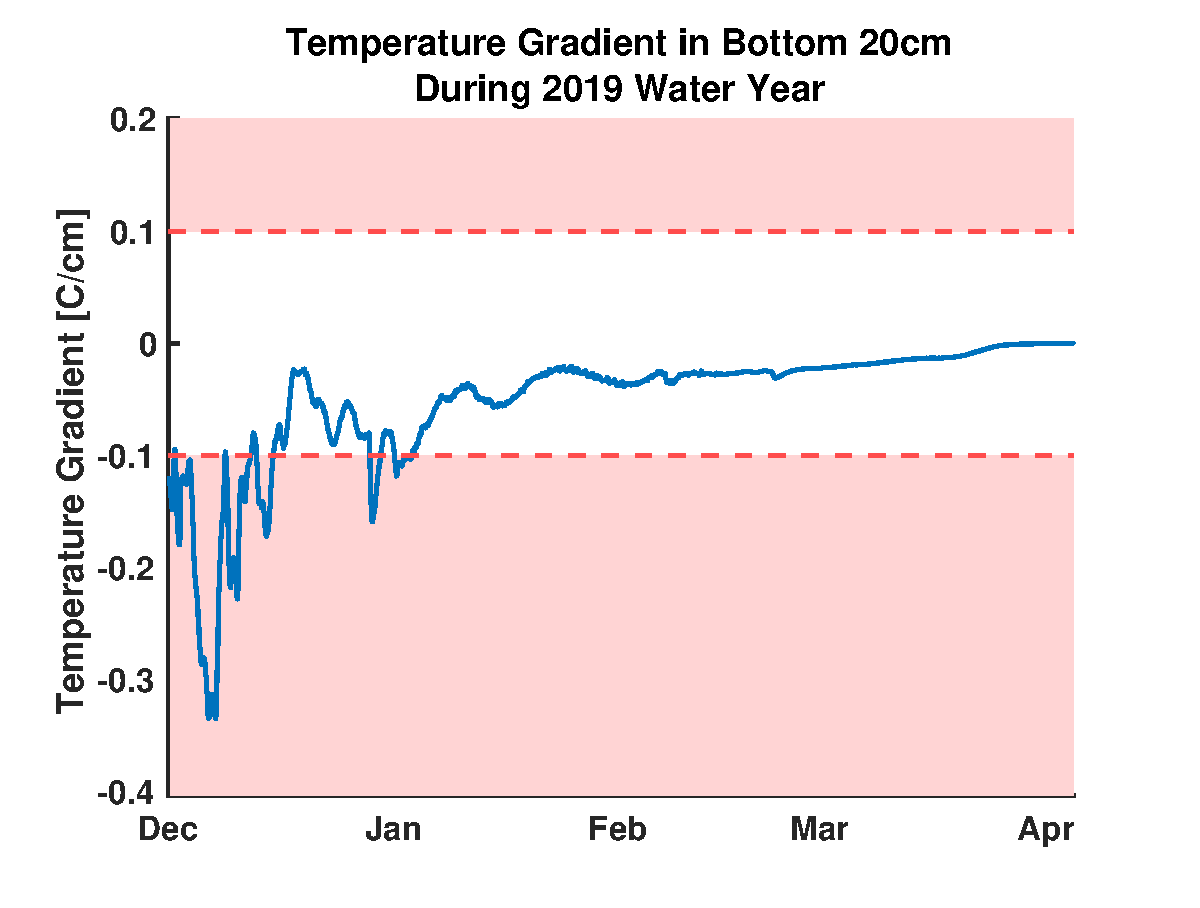
\includegraphics[width=0.7\linewidth]{figures/TempGrad/WY2019_L20_Grad.eps}
    \caption{Temperature gradient in lowest 20cm of snowpack during 2019 period of record. Gradients in the shaded red area are considered greater than critical and are facet forming.}
    \label{fig:WY2019_L20_Grad}
 \end{figure}
 
\begin{figure}[H]
    \centering
    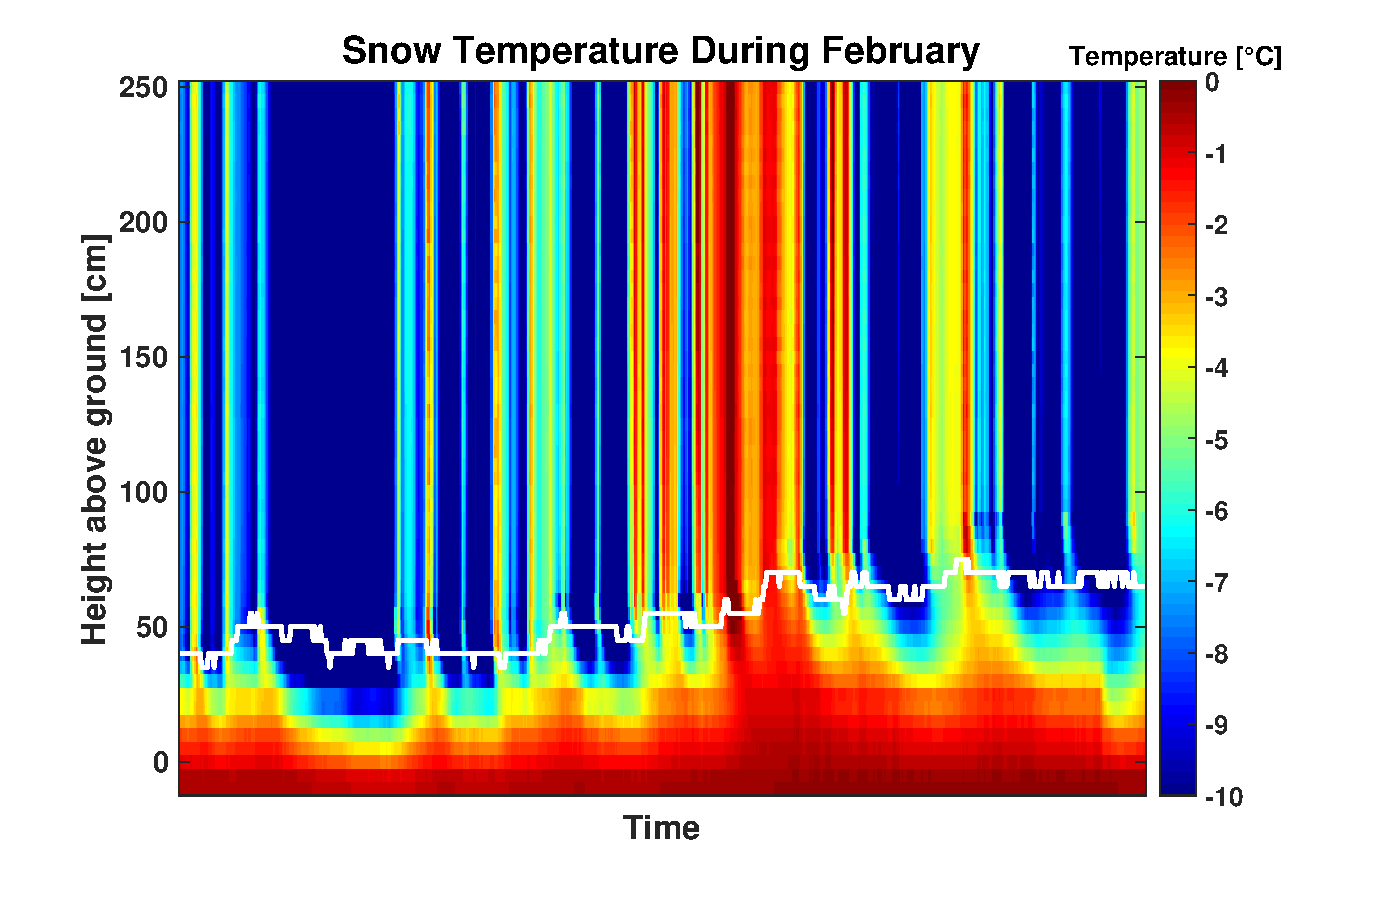
\includegraphics[width=0.95\linewidth]{figures/TempGrad/Dec_Heatmap.eps}
    \caption{Heatmap of data collected by BSTA during December. The solid white line indicates snow depth measured by the Banner Summit SNOTEl site.}
    \label{fig:Dec_U25_RDH}
 \end{figure}
 
  
  \begin{figure}[H]
    \centering
    \includegraphics[width=0.7\linewidth]{figures/TempGrad/Dec_U25_RDH.eps}
    \caption{Relative density histogram of temperature gradients in the upper 25cm of the snowpack during December. Gradients in the shaded red area are considered greater than critical and are facet forming.}
    \label{fig:Dec_Heatmap}
 \end{figure}
 
  \begin{figure}[H]
    \centering
    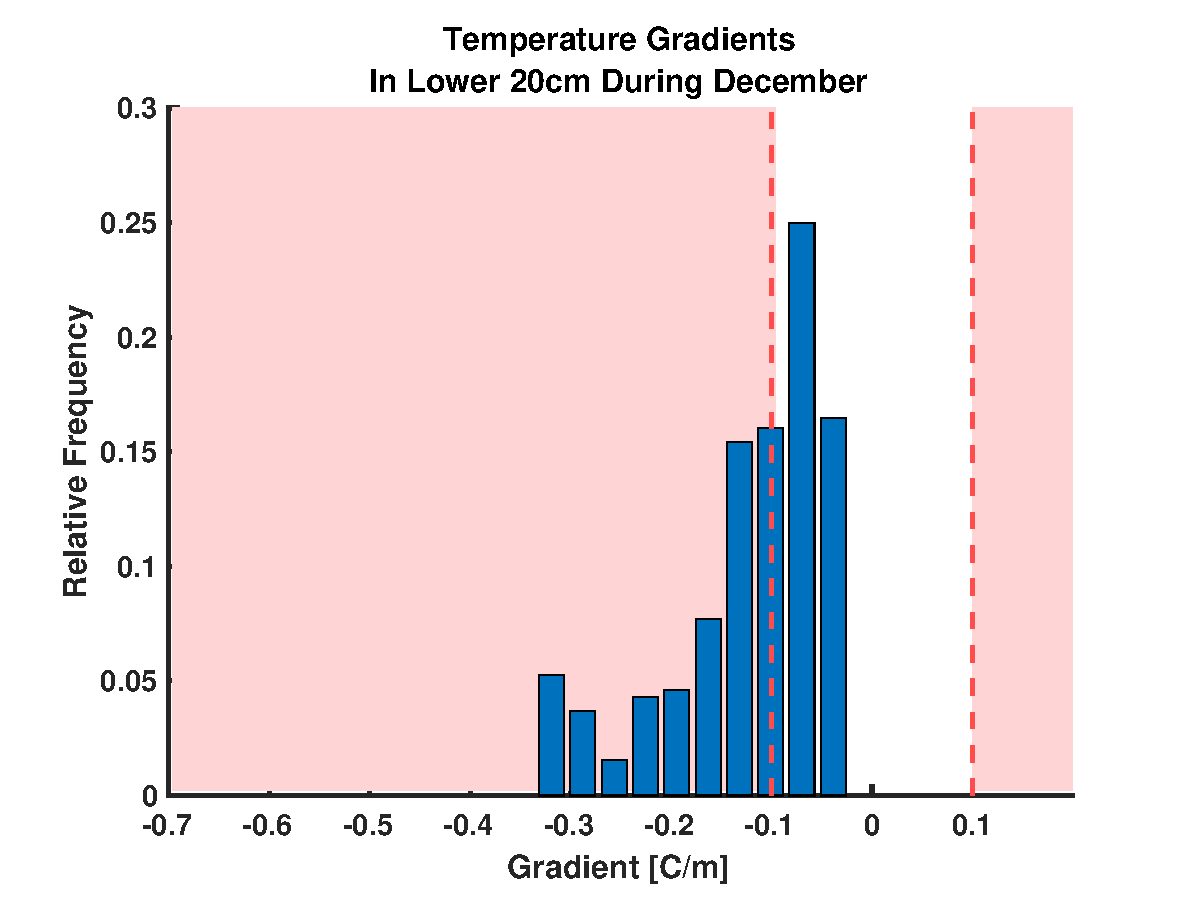
\includegraphics[width=0.7\linewidth]{figures/TempGrad/Dec_L20_RDH.eps}
    \caption{Relative density histogram of temperature gradients in the lowest 20cm of the snowpack during December.}
    \label{fig:Dec_L20_RDH}
 \end{figure}
 
  \begin{figure}[H]
    \centering
    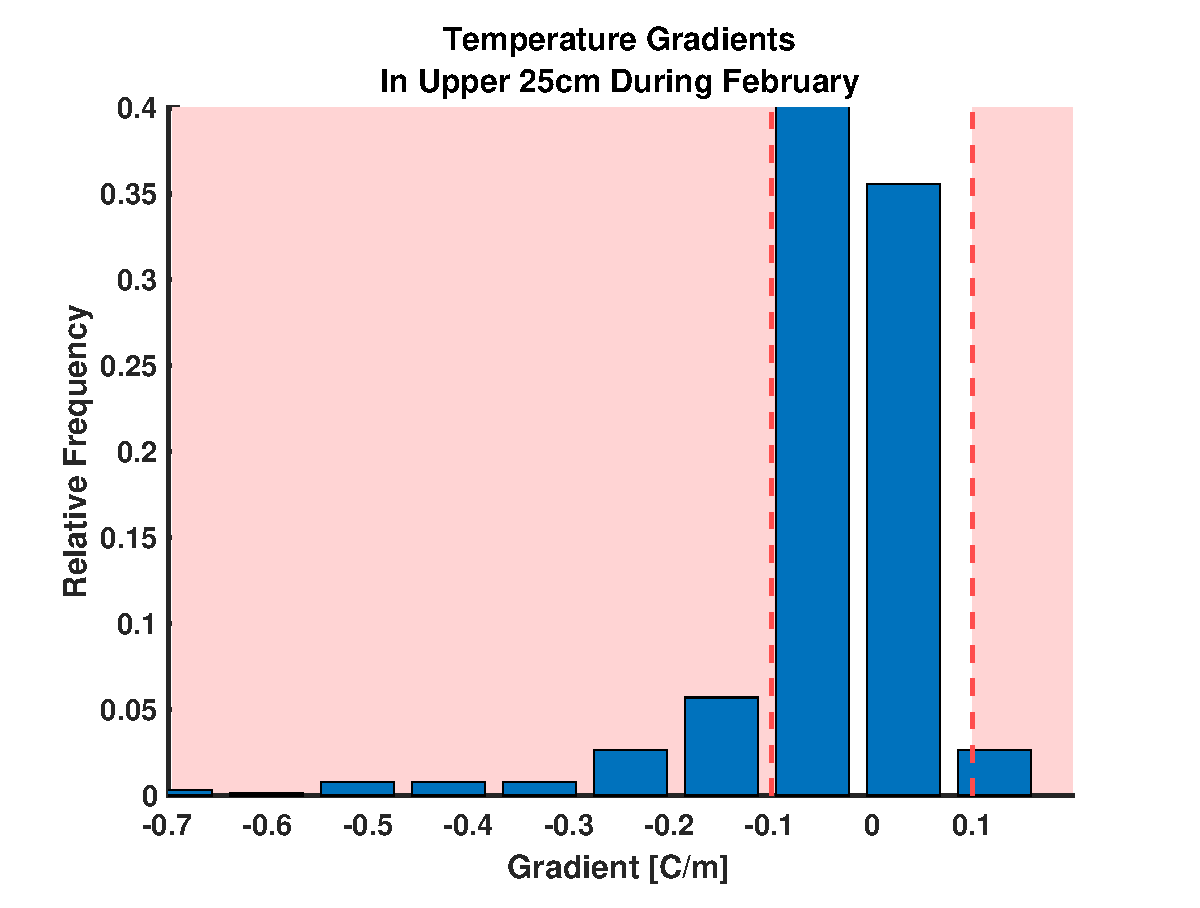
\includegraphics[width=0.7\linewidth]{figures/TempGrad/Feb_U25_RDH.eps}
    \caption{Relative density histogram of temperature gradients in the upper 25cm of the snowpack during February.}
    \label{fig:Feb_U25_RDH}
 \end{figure}
 
   \begin{figure}[H]
    \centering
    \includegraphics[width=0.7\linewidth]{figures/TempGrad/Feb_L20_RDH.eps}
    \caption{Relative density histogram of temperature gradients in the lowest 20cm of the snowpack during February.}
    \label{fig:Feb_L20_RDH}
 \end{figure}
 
   \begin{figure}[H]
    \centering
    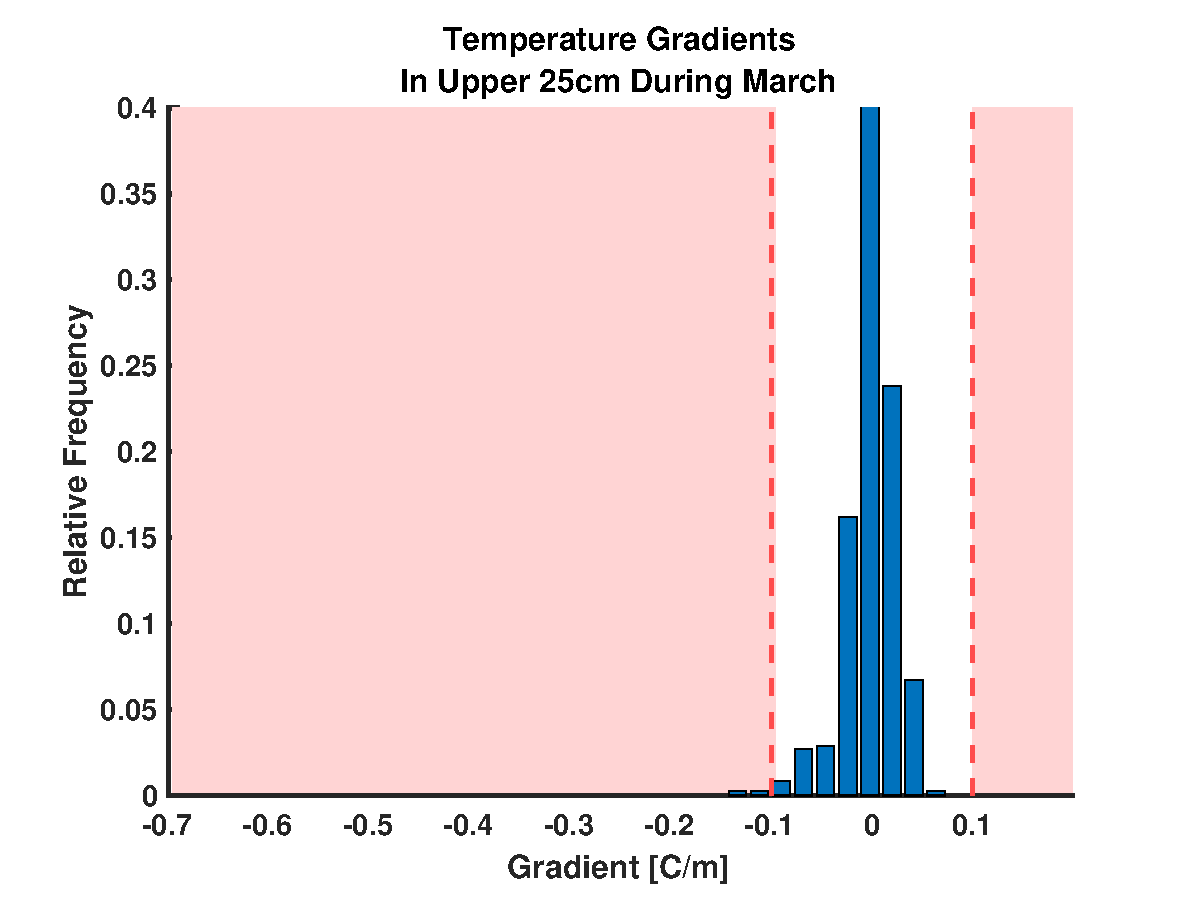
\includegraphics[width=0.7\linewidth]{figures/TempGrad/Mar_U25_RDH.eps}
    \caption{Relative density histogram of temperature gradients in the upper 25cm of the snowpack during March.}
    \label{fig:Mar_U25_RDH}
 \end{figure}
 
   \begin{figure}[H]
    \centering
    \includegraphics[width=0.7\linewidth]{figures/TempGrad/Mar_L20_RDH.eps}
    \caption{Relative density histogram of temperature gradients in the lowest 20cm of the snowpack during March.}
    \label{fig:Mar_L20_RDH}
 \end{figure}

\subsection{Stable Water Isotopes}
Early in the season, duplicate snow samples were taken from a single pit, but with ~0.5m horizontal spacing (Figure 7). This resulted in significant variations in stable isotopes near the top of the snowpack (Figure 8). The variation between duplicates was much lower in the bottom of the snowpack. Later in the season, Mar. 17th, triplicate samples were taken directly adjacent to each other (Figure 9) and the results suggest very little variation between triplicates. There are a number of things that might drive heterogeneity of snowpack stable isotopes, and this will be important to consider when further interpreting this dataset. Although there is spatial variability in stable isotopes, each storm should have a unique isotopic signature. Using field notes taken on storm layers within the snowpack, we can potentially measure the isotopic signature of each storm event and observe isotopic changes to the snow deposited by each storm.